\documentclass[a4paper]{ctexart}
%\usepackage[utf8]{inputenc}
\usepackage{amsmath, amsfonts, amsthm, graphicx, geometry, lipsum}
\usepackage{hyperref}
\hypersetup{
    colorlinks=true,
    linkcolor=blue,
    urlcolor=red,
    pdftitle={How to write a thesis},
    }
\usepackage{fancyvrb}
\usepackage{fancyhdr, lastpage}
\pagestyle{fancy}
\lhead{Trefor's awesome LaTeX guide}
\rhead{Sponsored by Overleaf!}
\cfoot{Page \thepage\ of \pageref{LastPage}}

\usepackage{etoolbox} %Use carefully!
\patchcmd{\chapter}{\thispagestyle{plain}}{\thispagestyle{fancy}}{}{}

\usepackage[Glenn]{fncychap}
%Options: Sonny, Lenny, Glenn, Conny, Rejne, Bjarne, Bjornstrup

\usepackage{xcolor}
\usepackage{tikz}
\usepackage[most]{tcolorbox}
\tcbset{colback=black!5!white,colframe=black!65!white} % globe set tclorbox

\newtcbtheorem{theo}%
  {Theorem}{}{theorem}
  
\usepackage{siunitx}
\usepackage{setspace}
\onehalfspacing

\usepackage[acronym]{glossaries-extra}
\setabbreviationstyle[acronym]{long-short}
\newacronym{dtb}{DTB}{Doctor Trefor Bazett}
\makeglossaries



\begin{document}

\tableofcontents

\newpage

%\chapter{Useful Packages}

\section{Hyperref} 
I want to link to my \href{https://www.youtube.com/watch?v=dQw4w9WgXcQ}{YouTube channel}. 



\section{fancyvbr}

\begin{Verbatim}[numbers=left, frame=single, formatcom=\color{red}]
\begin{center}
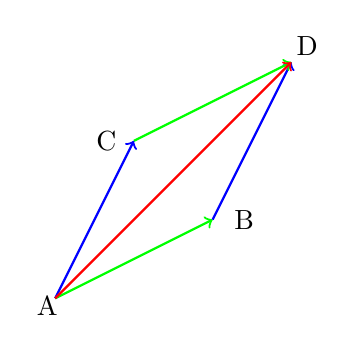
\begin{tikzpicture}

\draw[thick, green, ->] (0,0) -- (2,1);
\draw[thick, blue, ->] (2,1) -- (3,3);
\draw[thick, green, ->] (1,2) -- (3,3);
\draw[thick, blue, ->] (0,0) -- (1,2);
\draw[thick, red, ->] (0,0) -- (3,3);

\draw node at (-0.1, -0.1) {A};
\draw node at (2.4, 1) {B};
\draw node at (0.65, 2) {C};
\draw node at (3.2, 3.2) {D};

\end{tikzpicture}
\end{center}
\end{Verbatim}

\section{fncyhdr}

\section{etoolbox}

\section{GitHub}

\section{fncychap}

\section{Color}
Let's make {\color{red} this} be read.  \color{blue} This text will be blue until I change to a new colour like \color{black} black. 

\section{Tcolorbox}

\begin{tcolorbox}
This is a tcolorbox.
\end{tcolorbox}

\begin{tcolorbox}[colback=red!5!white,colframe=red!50!black,title=My nice heading]
This is a tcolorbox with a heading
\end{tcolorbox}

\begin{theo}{Like and Subscribe}{likesub}
For every person $x$, $x$ should like and subscribe. 

\end{theo}

\begin{theo}{Like and Subscribe}{likesub2}
For every person $x$, $x$ should like and subscribe. 

\end{theo}
\begin{tcolorbox}[title=My nice heading]
This  is  another  \textbf{tcolorbox}.
\tcblower
Here,  you  see  the  lower  part  of  the  box.
\end{tcolorbox}

\begin{tcolorbox}[colback=white!95!red,colframe=black!30!red,title=My  nice  heading]
This  is  another with sets  \textbf{tcolorbox}.
English news is a new education format. You will find articles and news from all over the world. English news is a school newspaper.
\tcblower
Here,  you  see  the  lower  part  of  the  box.
\end{tcolorbox}

\section{SI units}

\[5 kg m /s^2\]

\[5\ \mathrm{kg}\ \mathrm{m}/\mathrm{s}^2\]

\[5\ \si{kg.m/s^2}\]

\section{Setspace}

\lipsum[1-10]

\section{Glossaries and Acronyms}

I want to say \gls{dtb} to be long the first time and short the second \gls{dtb}. 






\printglossary[type=\acronymtype]
\end{document}
